{
\abnormalparskip{0pt}
\chapter{Discussion}
\label{cha:discussion}
}

This chapter discusses some of the possible extensions and directions one could
do with the work of the thesis. Apart from the more obvious possible
improvements, such as applying the lower bounds from \textcite{fampa2008} or prune
using the geometric properties \textcite{vanlaarhoven2013}, this chapter lists
some possible improvements and extensions for the new implementation.

\section{Concurrency}
\label{sec:concurrency}

Both the original and new implementation of the algorithm is implemented in a
sequential fashion. There also seems to be no literature concerned with making
the algorithm by \citeauthor{smith1992} concurrent.

Looking at \cref{fig:pprof} however may give an incitement to further
investigate the possibilities of making the algorithm concurrent. The figure
shows a CPU-time profile of the execution of the new implementation on a single
random instance (using \citeauthor{smith1992}'s iteration for optimization). As
can be seen, more than $50\%$ of the elapsed time is spent in the function with
the iteration (this is the time spent in the actual function, not waiting on
other function calls). Above that we see that if we count waiting for function
call that more than $80\%$ of the elapsed time was spent in the optimize
function. Here waiting on other function calls count towards the $80\%$. Making
especially the main loop concurrent and then running it concurrently on e.g.\
4--8 cores (which is a very common amount of cores in e.g.\ modern CPUs in of
any home desktop computer) could provide a very significant speedup.

\begin{figure}[htbp]
  \centering
  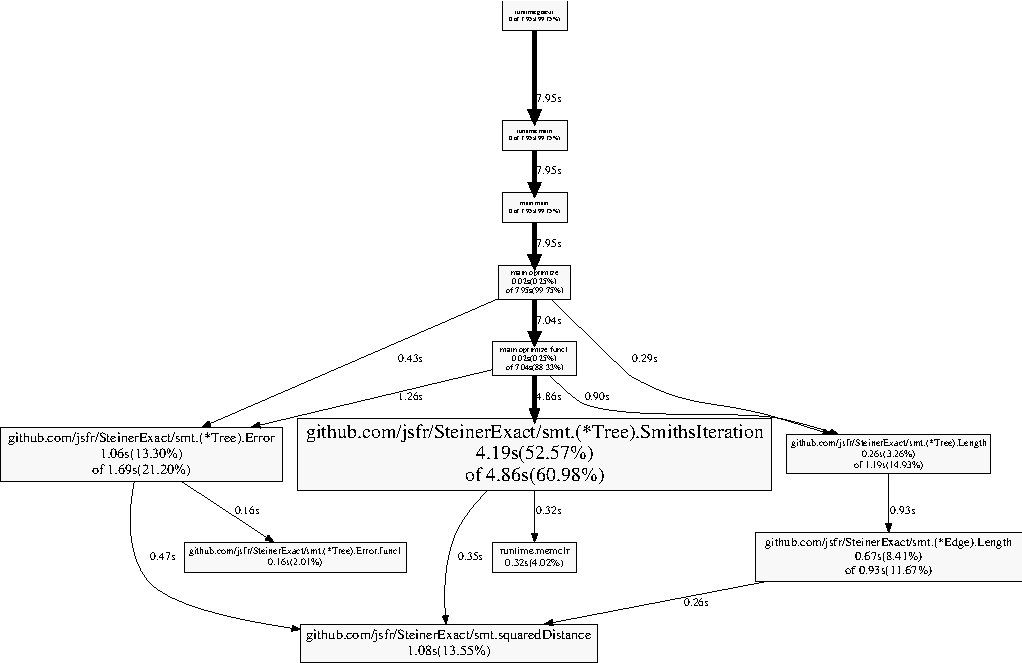
\includegraphics[width=\textwidth]{gfx/pprof001}
  \caption[CPU-time profile of a single execution]{CPU-time profile of the
    execution of the new implementation on a single random instance. The figure
    does not show the complete profile, as some of the smaller insignificant
    contributions have been remove for clarity. The initial entry-point of the
    program is the top box, showing the first function that is called in the
    program. Arrows indicate that the function in a box have called the
    function which the arrow points to. The times in the box shows the amount
    of seconds actually spent in the function (not waiting for other functions
    called within the function) of the amount of seconds spent in the function
    waiting for function calls as well.\label{fig:pprof}}
\end{figure}

We would then have to decide on some way of splitting up the problem instances.
One possible way of doing it would be to start one process for each half of the
children for the current topology vector. So say we currently have the topology
vector $[1, 2]$, we would then split this into two new processes, one which will
look at $[1, 2, 1]$ to $[1,2,4]$ and one which looks at $[1, 2, 5]$ to $[1, 2,
7]$. As long as we split in this fashion (no matter how many we decide to split
into) these can all be executed independently of each other, but would of course
benefit from synchronizing upper bounds. Thus we would make the upper bound with
a read-write lock which as mutual read (i.e.\ many can read the upper bound at
the same time) and exclusive write (i.e.\ only one can write a new upper bound
at a time). It is clear that the max number of splits
we can make, is the same number of edges we can split on every time we extend
the topology. Thus the max number the for the first split is $3$, foreach of
these $3$ we could split into $5$, and then for each of these into $7$, and so
forth.

Implementing a scheme as the one described above would allow us to both generate
and optimize multiple topology vectors in parallel which could provide a speedup
dependent on the number of cores available. Also, this approach would also
allow us to find upper bounds in parallel, which could mean that topologies
which we before were not able to prune, will now be pruned. Thus the shared
upper bound between processes could result in a further speedup.

The new implementation is as mentioned written in Go, which is a language that
makes implementing concurrency very straightforward. Thus extending the new implementation to
use concurrency could be done by refactoring a slightly changed version of
the main loop to a new function, and then spawn new goroutines. These should
then e.g.\ have a topology vector and some some boundaries for which part of the
descendants it should generate. Due to Go's way of making arrays, we would also
need to expand the \texttt{Tree} struct with a new function to clone the tree.
This would result in a slight slowdown, but more importantly it would require
the more memory equivalent again approximately to the number of running
processes.

\section{Propagating Changes in the Simple Iteration}
\label{sec:prop-chang-simple}

Currently the implementation of the simple iteration (using the analytical
solution) iterates through the Steiner points in a naive way when optimizing
them. It simply iterates through all Steiner points in the order they have been
added, and optimize them.

However consider adding the next terminal and a new Steiner point to a
topology. When adding the new Steiner point, we replace one edge with two, and
add one new edge. Thus all of the tree except for that one replaced edge, looks
exactly the same.

The order we could now choose to optimize the Steiner points in would be to
optimize the new Steiner point and let the change propagate from there. We
therefore next optimize any of the new Steiner points neighbors that are Steiner
points. If a Steiner point moves when it is optimized, we optimize any of
its neighbors that are Steiner points (and which has not yet been optimized). In
this way we propagate the optimization out through the tree from the new Steiner
point.

The reason this approach might be interesting is that we potentially avoid
optimizing whole sub-trees of the \ac{fst}, as if a Steiner point does not move,
nothing connected to the other side of it will move (assuming that part of the
tree was optimized during the previous topology).

Furthermore we also have that any Steiner point overlapping a terminal splits
the tree into two smaller sub-\acp{fst} and no change in one of the trees will
propagate to the other as long as the overlapping Steiner point does not move
away from the terminal\footnote{This property on sub-\acp{fst} also holds true for
\citeauthor{smith1992}'s iteration, and could therefore also be investigated
with this.}.

A further extension might be to not optimize out from the new Steiner point, but
to instead optimize out from the Steiner point which currently has the largest
error, under the assumption that the Steiner point with the largest error will
move the most and therefore cause its neighbors to move the most, thus
propagating the biggest change and leading to faster convergence.

\section{Initial Placement of Steiner Points}
\label{sec:init-plac-stein}

Currently both the original and new implementation place the Steiner points at the
perturbed centroid of their neighbors. However calculating the centroid is
about as computationally heavy as it is to calculate the Fermat-Torricelli point
using the analytical solution. Thus the implementation would probably benefit
from exchanging the perturbed centroid with the perturbed Fermat-Torricelli
point as a initial placement. The reasoning behind this is that all Steiner
points will be closer to their final optimal coordinates and thus we would need
fewer iterations in total.

\begin{table}[htbp]
  \centering
  \begin{tabular}{ccccccc}
    \toprule
         & \multicolumn{2}{c}{\footnotesize{\textit{Centroid}}}
         & \multicolumn{2}{c}{\footnotesize{\textit{Fermat-Torricelli point}}}
         & \multicolumn{2}{c}{\footnotesize{\textit{Ratio}}}                     \\
    $n$  & Iterations & Trees     & Iterations & Trees     & Iterations & Trees  \\
    \cmidrule(r){1-1}\cmidrule(lr){2-3}\cmidrule(lr){4-5}\cmidrule(l){6-7}
    $10$ & $73132.7$  & $4231.94$ & $58443.5$  & $1645.08$ & $0.80$     & $0.39$ \\ 
    $11$ & $307128$   & $18429$   & $238776$   & $6944.14$ & $0.78$     & $0.38$ \\
    $12$ & $1492050$  & $87869.2$ & $1122520$  & $32192.1$ & $0.75$     & $0.37$ \\
    \bottomrule
  \end{tabular}
  \caption[Perturbed centroid vs.\ perturbed Fermat-Torricelli point]{The table shows the average number of trees optimized and
    number of optimization iterations when placing the Steiner points at the perturbed
    centroid or the perturbed Fermat-Torricelli point initially. The data is for
    the cube instances used in \cref{sec:correctness}. \citeauthor{smith1992}'s iteration without terminal sorting was used. The last two columns
    show the ratio between the numbers for easier comparison. There are $50$
    instances of for each $n$.\label{tab:centroid-vs-fermat}}
\end{table}

To test the potential impact of this change a quick test was performed were the
use of the perturbed centroid was exchanged with the Fermat-Torricelli point,
perturbed exactly the same amount as the centroid was. The cube instances from
\cref{sec:correctness} were then run before and after the change, and the
average for the number of trees optimized and iterations for $n=10,11,12$ were
calculated. The results can be found in \cref{tab:centroid-vs-fermat}. Only
\citeauthor{smith1992}'s iteration (without terminal sorting) is used on the
data to be sure that the data is not affected by the sub-optimality seen in
\cref{sec:correctness} for the simple iteration\footnote{Furthermore the
  correctness test were performed again after the change just for good measure.
  This showed no new sub-optimal results, apart from those in the simple
  iteration already known.}. Furthermore were the correctness test also
performed after the change to ensure that no new sub-optimal result occurred. As
can be seen, at least for this data set, the program ran $\approx 20\%$ fewer
iterations, and optimized $\approx 60\%$ fewer trees. It therefore seems
worthwhile to make this very simple change, but more extensive performance tests
would probably have to be made.

%%% Local Variables:
%%% mode: latex
%%% TeX-master: "../../main"
%%% End:
